%----------------------------------------------------------------------------------------
%	PACKAGES AND THEMES
%----------------------------------------------------------------------------------------
\documentclass[aspectratio=169,xcolor=dvipsnames]{beamer}
\usetheme{SimplePlus}

\usepackage{hyperref}
\usepackage{graphicx} % Allows including images
\usepackage{booktabs} % Allows the use of \toprule, \midrule and \bottomrule in tables
\usepackage{amsmath, amsfonts, amssymb, amsthm, latexsym}
\usepackage[absolute,overlay]{textpos}

% \usepackage{authblk}
\usepackage{movie15}


%\usepackage{showkeys}

\usepackage{cancel}
%\usepackage{epsfig,cancel}


\usepackage{color}
% \usepackage{physics}

\usepackage[toc,page]{appendix}
%\usepackage{geometry}
\usepackage{braket}
\usepackage{bm}

\usepackage{graphicx}

\usepackage{tikz}

\usepackage{subfigure}

\usepackage{soul}

\usepackage{comment}


\let\Re\undefined

\let\Im\undefined

\DeclareMathOperator{\Re}{Re}

\DeclareMathOperator{\Im}{Im}


\DeclareMathOperator{\capa}{cap}

\DeclareMathOperator{\supp}{supp}

\DeclareMathOperator{\cl}{cl}


\newcommand{\ds}{\displaystyle}



%\newtheorem{algorithm}[theorem]{Algorithm}





\definecolor{shadecolor}{rgb}{0.95, 0.95, 0.86}

\usetikzlibrary{decorations.markings}



\def\red#1{\textcolor[rgb]{0.9, 0, 0}{#1} }

\def\yellow#1{\textcolor[rgb]{0.6, 0.5, 0 }{#1}}

\def\black{\special{color cmyk 0 0 0 1000}}

\def\cyan#1{\textcolor[rgb]{0,0.7,0.7}{#1}}

\def\blue#1{\textcolor[rgb]{0,0,1}{#1}}

\def\green#1{\textcolor[rgb]{0.2, 0.5,  0} {#1}}



\def\remove#1{\red{\cancel{#1}}}

\def\removelong#1{\red{ \small #1}}

\def\replace#1#2{\red{\cancel{{\hbox{\scriptsize  {$#1$}} }}}{\blue {#2}}}

%\def\insrt#1{\blue{#1}}

\def\insrt#1{\blue{#1}}



\def\be{\begin{equation}}

\def\ee{\end{equation}}

%

\def\bi{\begin{itemize}}

\def\ei{\end{itemize}}


%

\def\bea{\begin{eqnarray}}

\def\eea{\end{eqnarray}}

%

\def\bl{\begin{lemma}}

\def\el{\end{lemma}}

%

\def\bd{\begin{definition}}

\def\ed{\end{definition}}

%

\def\bp{\begin{proposition}}

\def\ep{\end{proposition}}

%


\def\br{\begin{remark}}

\def\er{\end{remark}}



%

\def\bt{\begin{theorem}}

\def\et{\end{theorem}}

%

\def\bc{\begin{corollary}}

\def\ec{\end{corollary}}

%

\def\ol{\overline}

\def\ra{\rightarrow}

\newcommand{\al}{\alpha}

%\newcommand{\bt}{\beta}

\newcommand{\de}{\delta}

\newcommand{\ga}{\gamma}

\newcommand{\G}{\Gamma}

\renewcommand{\O}{\Omega}

\renewcommand{\k}{\varkappa}

\renewcommand{\d}{\delta}

\newcommand{\D}{\Delta}

\newcommand{\e}{\varepsilon}

\renewcommand{\o}{\omega}

\newcommand{\g}{\gamma}

\newcommand{\la}{\lambda}

\newcommand{\si}{\sigma}

\newcommand{\ph}{\varphi}

\renewcommand{\part}{\partial}

\newcommand{\vn}{\varnothing}

\newcommand{\up}{\upsilon}

\newcommand{\coi}{C_0^{\infty}}

\newcommand{\ci}{C^{\infty}}

\newcommand{\ts}{\text{supp}\,}

\newcommand{\tB}{\tilde B}

\newcommand{\tss}{\text{singsupp}\,}

\renewcommand{\S}{\Sigma}

\newcommand{\rn}{\mathbb R^n}

\newcommand{\adx}{\vct\cdot x}

\newcommand{\Sn}{S^{n-1}}

\newcommand{\sg}{\text{sgn}}

\newcommand{\ibr}{\int_{\br}}

\newcommand{\brt}{\br^2}

\newcommand{\irt}{\int_{\brt}}

\newcommand{\ioi}{\int_0^{\infty}}

\newcommand{\iii}{\int_{-\infty}^{\infty}}

\newcommand{\isn}{\int_{\Sn}}

\newcommand{\fle}{f_{\Lambda\e}}

\newcommand{\CS}{{\mathcal S}}

\newcommand{\CD}{{\mathcal D}}

\newcommand{\CH}{{\mathcal H}}

\newcommand{\CB}{\mathcal B}

\newcommand{\bs}{\boldsymbol}

\newcommand{\Res}{\text{Res} \,}

\newcommand{\sign}{\rm{sign}}

\def\Rscr{\mathcal R}

\newcommand{\bu}{\bar{u}}

\newcommand{\sech}{\hbox{sech}}


\def\le{\left}

\def\ri{\right}

\def\B{\boldsymbol {\mathfrak B}}

\def \pa{\partial}

\def\C{{\mathbb C}}

%\def\L{\mathcal L}

\def\R{{\mathbb R}}

\def\N{{\mathbb N}}

%\def\z {{\mathbf z}}

\def\wh{\widehat}

\def\H{{\cal H}}

\def\Z{{\mathbb Z}}

\def\u{\mathfrak u}

\def\a{\alpha}

\def\b{\beta}

\def\g{\gamma}

%\def\gg{\mathfrak g}

\def\gt{\hat\gamma}

\def\vt{\hat v}

\def\gtb{\wh{\boldsymbol \gamma}}

\def\ct{\hat c}

%\def\d{\,\mathrm d}

\def\K{\mathcal K}

\def\m{\mu}

\def\l{\lambda}

\def\n{ {\nu}}

\def\Pot{\mathcal {P}}

\def\1{{\bf 1}}

\def\r{\rho}

%{\mathbf r}}

\def\c{ {\mathbf c}}

\def\s{ {\sigma}}

\def\t{ {\tau}}

\def\tsi{ {\tilde\sigma}}

\def\th{ {\theta}}

\def\w{{\mathbf w}}

\def\x{\xi}

\def\z{\zeta}

\def\ch{\mathbf {C}}

\def\sh{\mathbf {S}}

\def\hf{\frac{1}{2}}

\def \Th{\Theta}

\def\tf{\tilde\varphi}

\newcommand{\Iscr}{\mathcal I}
\newcommand{\Jscr}{\mathcal J}
\newcommand{\Bscr}{\mathcal B}
\newcommand{\Lscr}{\mathcal L}
\newcommand{\Wscr}{\mathcal W}
\newcommand{\Mscr}{\mathcal M}
\newcommand{\Nscr}{\mathcal N}
%\newcommand{\Rscr}{\mathcal R}

%----------------------------------------------------------------------------------------
%	TITLE PAGE
%----------------------------------------------------------------------------------------

\title[short title]{MAP 4113 Probability, Random Processes and Applications} % The short title appears at the bottom of every slide, the full title is only on the title page


\author{Instructor: Fudong Wang}

\institute[UCF] % Your institution as it will appear on the bottom of every slide, may be shorthand to save space
{
    Department of mathematics\\
    University of Central Florida
}
\date{} % Date, can be changed to a custom date


%----------------------------------------------------------------------------------------
%	PRESENTATION SLIDES
%----------------------------------------------------------------------------------------

\begin{document}

\begin{frame}
    % Print the title page as the first slide
    \vspace{-2cm}
    \titlepage
    \begin{center}
Lecture Notes for Fall2022 semester.
\end{center}
\end{frame}

\AtBeginSection[]
{
 \begin{frame}<beamer>
 \frametitle{Plan}
 \tableofcontents[currentsection]
 \end{frame}
}
\AtBeginSubsection[]
{
    \begin{frame}
        \frametitle{Table of Contents}
        \tableofcontents[currentsection,currentsubsection]
    \end{frame}
}
%------------Lecture 1------------------

%\section{Lecture 1: Combinatorial Analysis}

\subsection{Counting}
\begin{frame}{Problem of Counting}
    \begin{example}
    \begin{itemize}
        \item  How many possible outcomes after rolling a die?
        \pause
   \item  How many possible outcomes after flipping a coin twenty times?\pause 
   ($2^{20}=1048576
$)
\pause
  \item   What is max number of different 6-place plates? Using capital letters and numbers only.\pause 
  ($36^6=2176782336$)
  \pause
  \item How many different birthday combinations in the class? Only consider the day and month? What if consider day month and year?
    \end{itemize}
    \end{example}
\end{frame}

\begin{frame}{}
    \bt[Basic principle of counting]
    For a sequence of finite experiments, denoted by $(r_1,r_2,\cdots, r_N)$, each experiment $r_j$ can output $n_j$ results, then the total number of outputs is 
\begin{align}
\label{eq:prin of counting}
\prod_{j=1}^Nn_j:=n_1n_2\cdots n_N.
\end{align}
    \et
\end{frame}
\subsection{Permutation}
\begin{frame}{Permutation}
    \begin{itemize}
        \item Given an object of $n$ elements, an arrangement is called a permutation.
        \item For example, flipping coin twice, possible permutations are: HH,HT,TH,TT
        \item A sequence of letters $(a,b,c)$, there are 6 permutations: $$abc,acb,bac,bca,cab,cba.$$
    \end{itemize}
    \begin{block}{Questions}
    How many permutations for the sequence $\{a,a,b,c,c,d\}$? 
    \end{block}

\end{frame}
\begin{frame}{Permutation}
\bt[Basic permutation theorem]
\label{permuation theorem}
Suppose there are $n$ distinct objects, then the number of total permutations is 
\begin{align}
    n!:=n(n-1)(n-2)\cdots 2\cdot 1.
\end{align}
\et
\bt[General permutation theorem]
\label{gen permuation thm}
Suppose there $n$ objects with $n_1$ are alike, $n_2$ are alike,..., $n_r$ are alike, where $n_1+n_2+...+n_r=n$, then the total number of permutations are 
\begin{align}
    \frac{n!}{n_1!n_2!\cdots n_r!}
\end{align}
\et
    
\end{frame}
\begin{frame}{Permutation Model}
	\begin{itemize}
		\item Assign $n$ hats to $k$ people, how many ways?\pause
		\item If all hats are different, there are two cases: case 1, $k>n$, we will back to this later; case 2, $k\leq n$, then there are $n(n-1)\cdots (n-k+1)=\frac{n!}{k!}$ ways.
		\pause
		\item If there are $n_1$ white hats and $n_2$ black, suppose $n_1+n_2=n\geq k\geq \max\{n_1,n_2\}\}$, how many ways?
		\pause
		\item \red{A little bit hard.}  Symbolically, we have
		\[\sum_{k_1+k_2=k,k_1\leq n_1,k_2\leq n_2}\frac{n_1!n_2!}{k_1!k_2!}\]
	\end{itemize}
\end{frame}

\subsection{Combination}
\begin{frame}{Combination}
A \textit{combination} is a process by selecting objects from a given object. For example:
\begin{itemize}
    \item Consider the set $\{A,B,C,D\}$, how many different way of selecting 2 letters from the set? It's not hard to write down all possible combinations. They are $AB,AC,AD,BC,BD,CD$.
    \item \red{The order doesn't matter in dealing with combinations.}
    \item \blue{Question:} How to count the number of possible combinations in general, say, select $m$ items from $n$ \textbf{distinct} objects?
    \item Use the basic principle of counting!
\end{itemize}
    
\end{frame}

\begin{frame}{Combination}
Here is the reasoning. Suppose you have a set of $n$ distinct objects, you want to choose $m$ distinct objects from there. The first time, you have $n$ choices. The second time you will have $n-1$ choices. And the $m$-th time you only have $n-m+1$ choices. Then we can apply \red{ the basic principle of counting} to conclude that total number of (ordered) choices is 
\begin{align*}
    n(n-1)\cdots (n-m+1)=\frac{n!}{(n-m)!}.
\end{align*}
But, since we don't care the order of the outcomes, it follows the number of different way of picking $m$ objects is
\begin{align*}
    \frac{n!}{m!(n-m)!}.
\end{align*}
    
\end{frame}

\begin{frame}{Hat problem}
	\begin{itemize}
		\item Back to the hat problem, now let us consider $n< k$ case.
		\item First we need select $k-n$ people from the $k$ people group, that's \red{stage one}.
		\item \red{Stage two} is assign the $n$ hats to the rest $n$ people.
		\item Using the basic counting principal, we have
		\[\binom{k}{k-n}n!=\frac{k!}{(k-n)!}\]
	\end{itemize}
\end{frame}

\begin{frame}{Combination}
A notation will be introduced to denote the number of combination:
\[
\binom{n}{m}:=\frac{n!}{m!(n-m)!}.
\]
Using this notation, we can state a useful algebra theorem
\bt [The Binomial theorem]
$$
    (x+y)^n=\sum_{k=0}^n\binom{n}{k}x^ky^{n-k}.
$$
\et 
\bc By choosing $x=y=1$, we get 
$$
    2^n=\sum_{k=0}^n\binom{n}{ k}.
$$
\ec
\end{frame}

\begin{frame}{A combinatorial proof}
\begin{proof}
    Let's consider two sets $\{x_1,\cdots,x_n\}$and $\{y_1,\cdots,y_n\}$, consider the following product
    \[(x_1+y_1)(x_2+y_2)\cdots(x_n+y_n).\]
    To expand this product, we basically select a factor from each bracket, and the factor is of the form
    $
        z_1z_2\cdots z_n,
$
    where $z$ could be $x$ or $x$. Each factor represents a way of selecting objects. Since the order doesn't matter, the number of way of selecting $k$ $x$ and $n-k$ $y$ is given by $\binom{n}{k}$. Now, let all $x_i=x$ and $y_i=y$, we get
    \begin{align*}
        (x+y)^n=\sum_{k=0}^n\binom{n}{k}x^ky^{n-k}.
    \end{align*}
\end{proof}
    
\end{frame}

\begin{frame}{A remark}
	\textbf{Remark:} Combination doesn't feel the order, thus needs to divide by permutations. To get rid of labels is equivalent to eliminating the order, thus, we can consider
	\[\binom{n}{m}=\frac{n!}{m!(n-m)!}\]
	as selecting $m$ $x$ and $n-m$ $y$ and then divide by their permutations $m!$ and $(n-m)!$ respectively. And this can be generalized to multi-variables.
\end{frame}

\begin{frame}{Combination}
    \bt[The multinomial theorem]
\label{multinomial thm}
\begin{align}
    \le(\sum_{k=1}^rx_k\ri)^n=\sum_{n_1+n_2+\cdots+n_r=n}\binom{n}{ n_1,n_2,...,n_r}x_1^{n_1}x_2^{n_2}\cdots x_r^{n_r}.
\end{align}
The sum on the right hand side is over all non-negative integer valued vectors $(n_1,...,n_r)$ such that $\sum_{k=1}^rn_k=n$. 
\et

\textbf{Question:} Find the Taylor expansion formula for multi-variable functions and understand the meaning of the Taylor coefficients. Write down the Taylor expansion (near origin) for the following functions:
\begin{align*}
    e^{x+y},\quad \sin(x+y),\quad \ln(x^2+y^2+1).
\end{align*}
\end{frame}
\subsection{Practice}
\begin{frame}{Practice Problems}
\begin{itemize}
    \item How many 5-card poker hands are there? No jokers.
    \pause
    \item If 8 identical apples are to be divided among 4 students, how many divisions are possible? What if each student must at least receive one?
    
    \item How many non-negative integer solutions of the following equation: $x+y+z=100$?
   
    \item Number of non-negative solutions to the following inequality:
    \[\sum_{i=1}^n x_i\leq k?\]\pause
     \item Show $\sum_{k=1}^n k\binom{n}{k}=n\cdot 2^{n-1}.$
    \item Show $\sum_{k=1}^n k^2\binom{n}{k}=n(n+1)\cdot 2^{n-2}.$
\end{itemize}
    
\end{frame}

\begin{frame}{More Problems}

\begin{columns}
\begin{column}{0.5\textwidth}
\begin{figure}[ht]
    \centering
    
\begin{tikzpicture}
\draw (0,0) node[anchor=north east]{A} grid (6,4) node[anchor=south west]{B};
 \node at (0,0) [circle,fill,inner sep=1.5pt]{};
 \node at (6,4) [circle,fill,inner sep=1.5pt]{};
 \draw[thick,->,red] (0,0) -- (2,0);
 \draw[thick,->,red] (2,0) -- (2,2);
 \draw[thick,->,red] (2,2) -- (5,2);
 \draw[thick,->,red] (5,2) -- (5,4);
 \draw[thick,->,red] (5,4) -- (6,4);
\end{tikzpicture}

    \caption{An exmaple path from A to B.}
    \label{fig: Counting path}
\end{figure}
\end{column}
\begin{column}{0.5\textwidth}
\textbf{Question:} A bug is walking from A to B, and it can only move up or right, the figure shows a possible path from A to B. How many possible different ways from A to B? The coordinate of A and B are $(0,0)$ and $(6,4)$ respectively. \red{How to generalize it to arbitrary two points? What if the bug must pass a provided point, say $(2,2)$, how many ways it can possible go from A to B? }
\end{column}
\end{columns}
\end{frame}
\subsection{Summary}
\begin{frame}{Summary}
\begin{enumerate}
    \item If the elements are \textbf{reusable}, then \textbf{Basic principal of counting}; Else
    \item If there are $n$ distinct objects, then \textbf{Permutation}; Else
    \item if there are repeating objects, then \textbf{General permutation}; Else
    \item if \textbf{Order} doesn't matter, then standard \textbf{combination}; Else
    \item Combination \textbf{times} permutation.
\end{enumerate}
    
\end{frame}

\subsection{Homework}
\begin{frame}{Homework 1 }
	\begin{columns}
		\begin{column}{0.5\textwidth}
			\begin{itemize}
				\item Ross Chapter I Problems: 3, 15, 19, 31
				\item Ross Chapter I Theoretical Exercises: 11, 12, 14 
				\item Given a pack of 52 standard cards, selecting 5 cards, how many ways to get a pair? What about three of a kind?
				\item Simplify $\sum_{k=1}^n k^3\binom{n}{k}$, and prove it. 
			\end{itemize}
		\end{column}
	\begin{column}{0.5\textwidth}
		\begin{itemize}
			
			\item (Whole line 1D Random Walk) Consider a particle is moving on the real integer line ($\cdots,-3,-2,-1,0,1,2,3,\cdots$), starting at 0, each step it can move left/right one unit, after 10 moves, how many different paths can happen? 
			\item (Half line 1D Random Walk) Now consider starting point at 0, and the domain is now $\Z_+\cup \{0\}=\{0,1,2,3,\cdots\}$, how many paths of length 10?
			\item For the half line 1D RW, what if the starting point is $x\in \Z_+$, how many paths of length 10?
		\end{itemize}
	\end{column}
	\end{columns}
\end{frame}

\section{Lecture 2}

\subsection{What Is Probability?}

\begin{frame}{What is probability?}
	\begin{itemize}
		\item \textbf{As a limit of \textit{relative frequency}:}
		\[\lim_{\# \text{ of experiments}\ra \infty}\frac{\# \text{ of occurring}}{\# \text{ of experiments}}.\]
		\item \textbf{As a person's belief:} Just a feeling base on your own experience.
		\item \textbf{A function defined on events.}
		\item Many other answers$\cdots$
	\end{itemize}
\end{frame}



\subsection{Sample Space and Events}
\begin{frame}{Sample Space and Events}
	Before we define probability, we need first define so-called \textbf{sample space and events.}
	\begin{itemize}
		\item The \textbf{mutually exclusive} outcomes of a random experiment will be called \textbf{elementary events}, usually denoted by $\omega$.
		\pause
		\item  The set of all elementary events will be called the \textbf{sample space}, denoted by $\Omega$. 
		\item An \textbf{event} is a subset of the sample space.\pause
		\item \textbf{Example:} The experiment of flipping a coin twice. The sample space is
		\be
		\Omega=\{HH,HT,TH,TT\}.\nonumber
		\ee
		\item Here are several examples of events:
		\begin{itemize}
			\item At least one time is head :$\{HH,HT,TH\}$.
			\item Exactly one head: $\{HT,TH\}$.
		\end{itemize}
	\end{itemize}
\end{frame}
\begin{frame}{More Examples}
	
	\begin{columns}
		\begin{column}{0.65\textwidth}
				\begin{figure}[HT]
				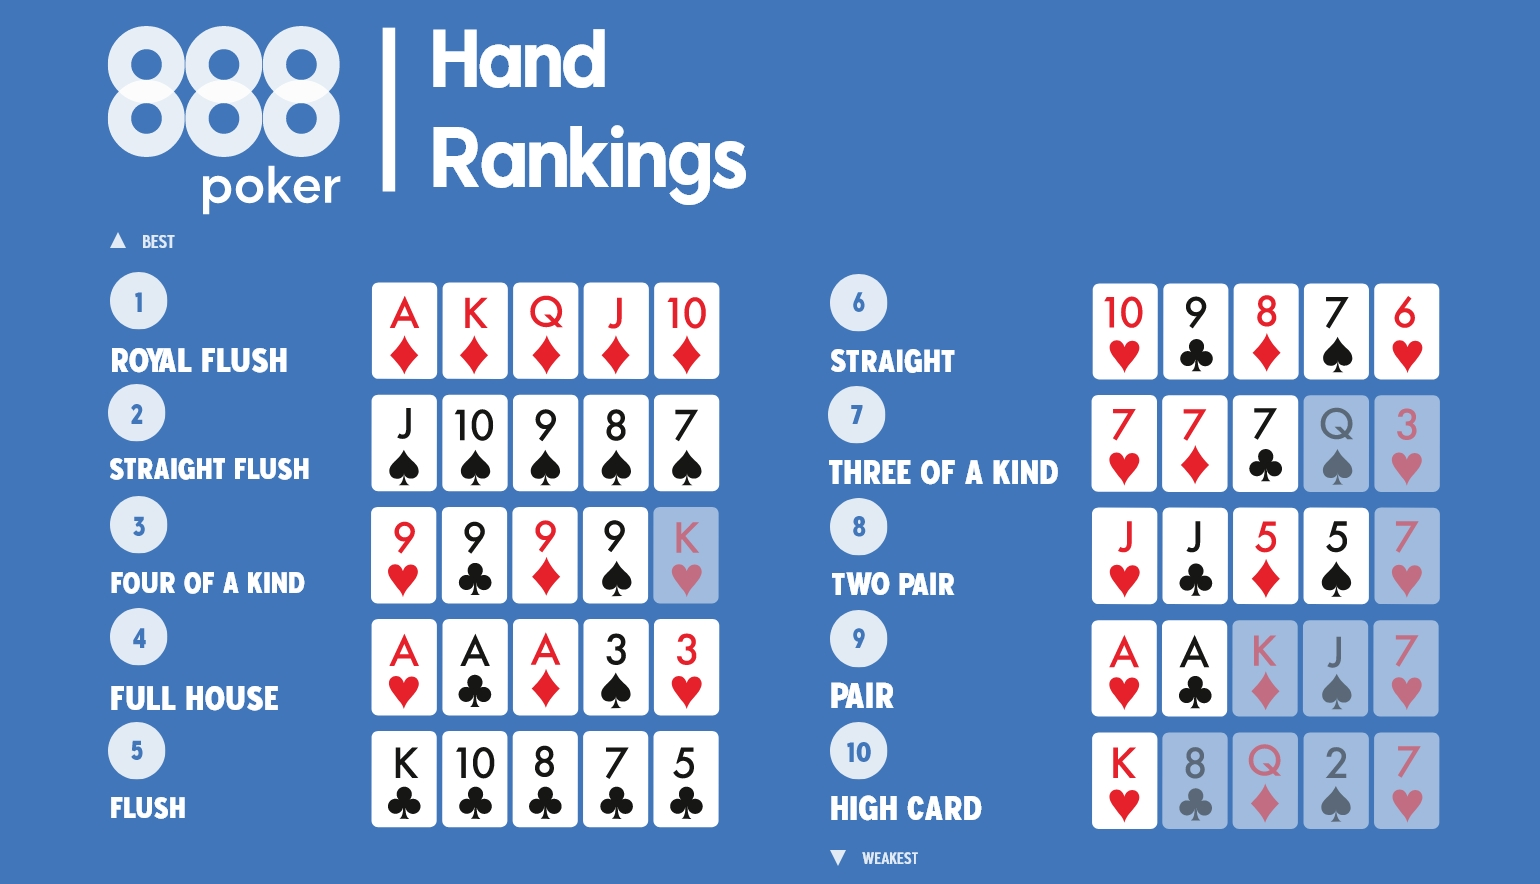
\includegraphics[width=0.8\textwidth]{poker.jpg}
			\end{figure}
		\end{column}
	\pause
	\begin{column}{0.3\textwidth}
		\begin{itemize}
			\item Each hand represents an event. (A set that satisfies the requirement.)\pause
			\item Are they \textbf{mutually exclusive}? (Discussion)
			\item How to describe the relations among different events? 
		\end{itemize}
	\end{column}
	\end{columns}
\end{frame}

\subsection{Theory of Set}

\begin{frame}{Use the language of set to describe events}
	\bd
		\begin{itemize}
			\item The event $E\cup F$ is called the union of events $E$ and $F$, which means at least one of the events occur.
			\item  The event $E\cap F$ is called the intersection of $E$ and $F$, conventionally denoted by $EF$, which means $E$ and $F$ occur at the same time.
			\item  The event $\overline E$ stands for the event that $E$ hasn't occurred. 
			\item $E\subset F$ means the occurrence of $E$ implies occurrence of $F$.
			\item $E-F$ means event $E$ occurs but $F$ doesn't occur.
		\end{itemize}
		
	\ed
\end{frame}

\begin{frame}{Properties}
	Here are some fundamental properties from the set theory:
	\begin{enumerate}
		\item $E\cup F=F\cup E$ and $EF=FE$.
		\item $(E\cup F)\cup G=E\cup (F\cup G)$ and $(EF)G=E(FG)$.
		\item $(E\cup F)G=EG\cup FG$ and $EF\cup G=(E\cup G)(F\cup G)$.
		\item (\textbf{DeMorgan's laws}) $\overline{E\cup F}=\overline E\cap \overline F$. [\textbf{Exercise}: Extend it to $n$ events!]
	\end{enumerate}
Let's see two exercises:
\begin{enumerate}
	\item Find $X$ such that 
	\begin{align*}
		\ol{(X\cup A)}\cup \ol{(X\cup \ol A)}=B.
	\end{align*}
\item Interpret the following relations involving events $A$,$B$ and $C$:
a). $AB=A$; b). $ABC=A$; c). $A\cup B\cup C=A$.
\end{enumerate}

\end{frame}

\begin{frame}{Venn Diagrams}
	\begin{figure}[ht]
		\centering
		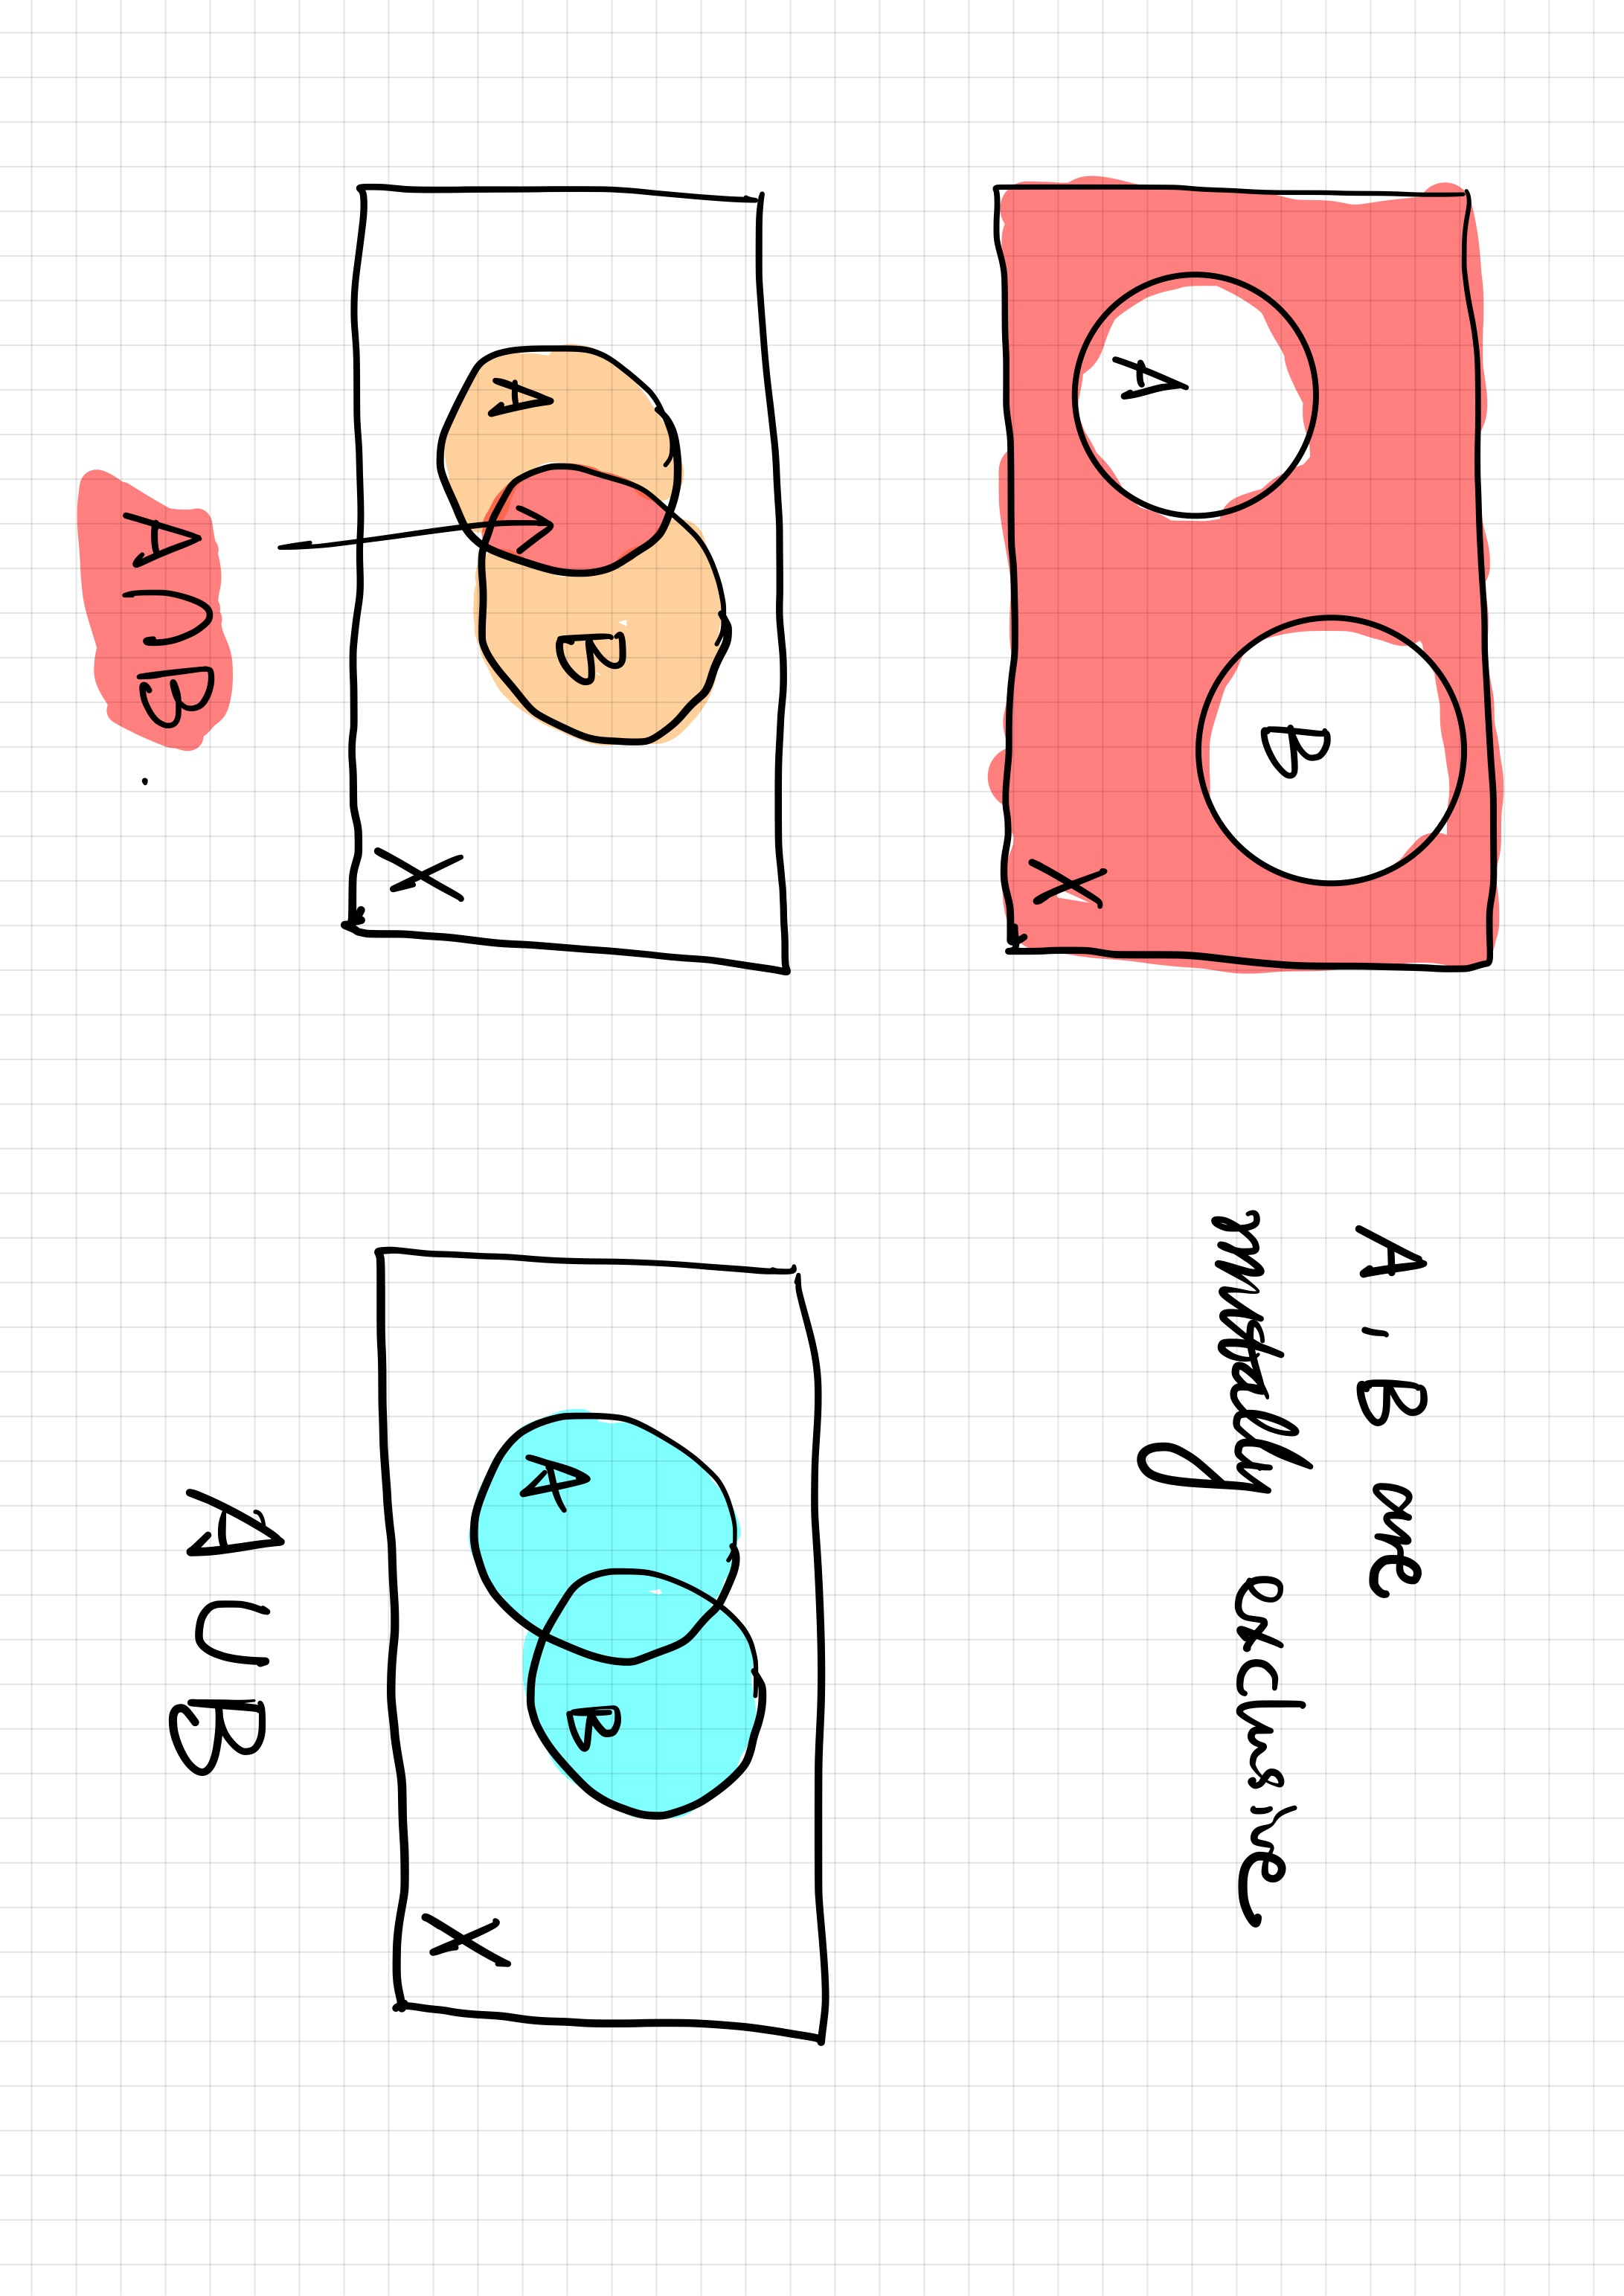
\includegraphics[angle=90,width=0.75\textwidth]{venndiag.jpg}
	\end{figure}
\end{frame}

\begin{frame}{Proof of the DeMorgan's Laws}
	\begin{proof}
	Let $x\in \overline{E\cup F}$, then $x\notin E\cup F$, that is to say $x\notin E$ and $x\notin F$. In notation it means $x\in \ol E$ and $x\in \ol F$ which implies $x\in \ol E \cap \ol F$, the right hand side.\pause  Thus we have shown 
	\[\overline{E\cup F}\subset \ol E \cap \ol F.\]\pause
	On the other hand, one can see that the above argument is reversible  and this completes the identity.
\end{proof}
\end{frame}

\subsection{Axioms of Probability}

\begin{frame}{What is Probability again?}
	One \textbf{intuitive way} to define the probability of an event is as the limit of relative frequency:
	\begin{align}
		P(E)=\lim_{n\ra \infty}\frac{n(E)}{n},
	\end{align}
where $n(E)$ denotes the time  event $E$ occurs after $n$ trails. From this definition, we have
\begin{enumerate}
	\item $0\leq P(A)\leq 1$ for any event $A$. And $P(\Omega)=1$.
	\item 	Provided that $A,B$ are mutually exclusive.
	\[P(A\cup B)=P(A)+P(B)\]
	\item Moreover, for mutually exclusive events $\{A_k\}_{k=1}^n$, we have
	\[P(\cup_{k=1}^n A_k)=\sum_{k=1}^nP(A_k),\quad (\text{addition law for probabilities.})\]

\end{enumerate}
\end{frame}
\begin{frame}{Definition of Probability}
	\bd
	Let $P$ be a function that assigns a real value to each events and satisfies the following three axioms: Let $\Omega$ be the sample space,
	\begin{enumerate}
		\item $0\leq P(A)\leq 1$
		\item $P(\Omega)=1$
		\item If events $\{A_k\}_{k\geq 1}$ mutually exclusive, we have
		$
			P(\cup_{k\geq 1}A_k)=\sum_{k\geq 1} P(A_k).
	$
	\end{enumerate}
Such function $P$ is called a probability. [\red{Existence?}]
	\ed
	\begin{example}
		Flip coins once. Let $\Omega=\{H,T\}$. We define $P(\{H\})=2/3$ and $P(\{T\})=1/3$. Then such $P$ is a probability.\pause \red{Design a fair game using this coin.}
	\end{example}	
\end{frame}

\begin{frame}{Some properties of a probability}
	\bt
	For any events $A,B$, the following relations hold:
	\begin{align}
		& P(A-B)=P(A)-P(AB),\\
		& P(A\cup B)=P(A)+P(B)-P(AB),\\
		& P(A)\leq P(B) \quad if\quad A\subset B.
	\end{align}
	\et
	\begin{proof}
		Use addition law for probabilities (\textbf{the third axiom of probability}).
	\end{proof}
\end{frame}

\begin{frame}{An important theorem:  The inclusion-exclusion identity}
	\bt
	[The inclusion-exclusion identity] Let $E_1,...,E_n$ be $n$ arbitrary events, then
	\begin{align*}
		P(\cup_{i=1}^n E_i)=\sum_{r=1}^n (-1)^{r+1}\sum_{i_1<i_2<...<i_r}P(E_{i_1}\cdots E_{i_r}).
	\end{align*}
	\et
	\begin{example}
		Flip a fair coin twice. Then $\Omega=\{HH,HT,TH,TT\}$. Let $E_1=\{\text{at least one $H$}\}$ and $E_2=\{\text{at least one $T$}\}$.  Then $P(E_1\cup E_2)=P(E_1)+P(E_2)-P(E_1E_2)=3/4+3/4-1/2=1.$
		
		Note Here for a fair coin, $P(A)=|A|/|\Omega|$.
	\end{example}
	
	
\end{frame}


\begin{frame}{Proof of the inclusion-exclusion identity}

			We will prove it by math induction. $n=1$ is trivial and $n=2$ is proved in the previous theorem. Suppose the statement is true for $n$ events, let's show it is also true for $n+1$ events. In fact, 
			\begin{align*}
				P(\cup_{i=1}^{n+1} E_i)&=P(\cup_{i=1}^n E_i\cup E_{n+1})\\
				&=P(\cup_{i=1}^n E_i)+P(E_{n+1})-P((\cup_{i=1}^n E_i)E_{n+1})\\
				&=\sum_{r=1}^n (-1)^{r+1}\sum_{1\leq i_1<i_2<...<i_r\leq n}P(E_{i_1}\cdots E_{i_r})+P(E_{n+1})\\
				&-\sum_{r=1}^n (-1)^{r+1}\sum_{1\leq i_1<i_2<...<i_r\leq n}P(E_{i_1}\cdots E_{i_r}E_{n+1}).
			\end{align*}

		

\end{frame}

\begin{frame}{Proof of the inclusion-exclusion identity}
	Since for any $r\leq n$, we have
	\begin{align*}
		&(-1)^{r+1}\sum_{1\leq i_1<i_2<...<i_r\leq n}P(E_{i_1}\cdots E_{i_r})- (-1)^{r}\sum_{1\leq i_1<i_2<...<i_{r-1}\leq n}P(E_{i_1}\cdots E_{i_r}E_{n+1})\\
		&=(-1)^{r+1}\sum_{1\leq i_1<i_2<...<i_r\leq n+1}P(E_{i_1}\cdots E_{i_r}).
	\end{align*}
	Thus, we have
	\begin{align*}
		P(\cup_{i=1}^{n+1} E_i)&=\sum_{r=1}^n (-1)^{r+1}\sum_{1\leq i_1<i_2<...<i_r\leq n+1}P(E_{i_1}\cdots E_{i_r})\\
		&+(-1)^{n+2}\sum_{1\leq i_1<i_2<...<i_n\leq n}P(E_{i_1}\cdots E_{i_r}E_{n+1})\\
		&=\sum_{r=1}^{n+1} (-1)^{r+1}\sum_{1\leq i_1<i_2<...<i_r\leq n+1}P(E_{i_1}\cdots E_{i_r}).
	\end{align*}
\end{frame}
\begin{frame}{A remark on the inclusion-exclusion identity}
	For simplicity, one can denote
	\begin{align*}
		P_k=\sum_{1\leq i_1<...<i_k\leq n}P(E_{i_1}...E_{i_k}).
	\end{align*}
	Then one can write the inclusion-exclusion identity as follows:
	\begin{align*}
		P(\bigcup_{i=1}^n E_i)=P_1-P_2+P_3-...+(-1)^{n+1}P_n.
	\end{align*}

\end{frame}

\subsection{Practice}

\begin{frame}{Practice Problems}
	 \begin{example}
		[Coincidences] 
		\label{Coincidences exmaple}
		Suppose $n$ students put their ID cards inside a box, then draw randomly from the box, what is the probability that at least one student get its own ID card?
	\end{example}
\textbf{Solution:} Apply inclusion-exclusion identity. Denote $A_k$ the event that $k$-th student gets his own ID. We need to compute 
\begin{align*}
	P(\bigcup_{k=1}^nA_k).
\end{align*}\pause
Let's first compute $P_1$. In fact, since $P(A_k)=\frac{(n-1)!}{n!}$, we obtain
\begin{align*}
	P_1=\binom{n}{1}\frac{(n-1)!}{n!}.
\end{align*}
\end{frame}
\begin{frame}{Cont.}
Similarly, one can show that
\begin{align*}
	P_m=\binom{n}{m}\frac{(n-m)!}{n!}=\frac{1}{m!}.
\end{align*}
Thus, from the inclusion-exclusion identity, we have
\begin{align*}
	P(\bigcup_{k=1}^n A_k)=\sum_{m=1}^n(-1)^{m+1}\frac{1}{m!}.
\end{align*}

\red{What happens if $n\ra\infty$?}
\end{frame}

\begin{frame}{Limiting probability}
	If we let $n\ra \infty$, we will get
	\begin{align}
		P(\bigcup_{k=1}^\infty A_k)=1-\frac{1}{e}\approx 0.63212055882.
	\end{align}
	Using Taylor's theorem, we have
	\begin{align*}
		P(\bigcup_{k=1}^n A_k)=1-\frac{1}{e}+R_n,
	\end{align*}
	where the error term is bounded as follows
	\begin{align*}
		|R_n|\leq \frac{c}{(n+1)!}.
	\end{align*}
\end{frame}

\begin{frame}{More Practice}
	If $n$ people are in a room, what is the probability that no two of them were born at the same date of the year (ignoring Feb 29th)?\pause
	\begin{proof}
		The size of the sample space is $365^n$. The event can also be easily computed: that is \red{why?}
		\[\frac{365!}{(365-n)!}\]\pause
		Thus, suppose each outcome is equally likely, the probability is 
		\[\frac{365!}{(365-n)!(365)^n}\]
	\end{proof}
\end{frame}
\begin{frame}{Cont.}
	%\includemovie{1cm}{1cm}{Birthday.gif}
	\begin{figure}[ht]
		\centering
		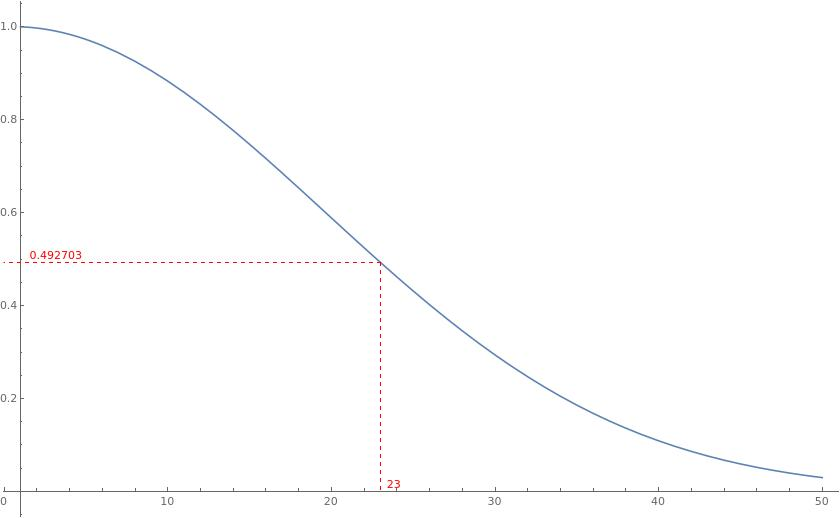
\includegraphics[width=0.8\textwidth]{birthday23.jpeg}
	\end{figure}
\end{frame}

\subsection{Homework}

\begin{frame}{Homework}
	\begin{enumerate}
		\item [$\bigstar$] Ross Chapter 2, Problem: 2, 4, 15, 27, 41
		\item [$\bigstar$] Ross Chapter 2, Theoretical Exercises: 4, 10, 8, 16, 19,
	\end{enumerate}
\end{frame}








%------------------------------------------------



\end{document}